\documentclass{standalone}
\usepackage{amsmath}
\usepackage{amssymb}
\usepackage{amsfonts}
\usepackage{xcolor}
\usepackage{tikz}
\usepackage{tkz-euclide}
\usetikzlibrary{calc}
\usetikzlibrary{patterns,arrows.meta}
\usetikzlibrary{shadows}
\usetikzlibrary{external}
\usepackage{pgfplots}
\pgfplotsset{compat=newest}
\usepgfplotslibrary{statistics}
\usepgfplotslibrary{fillbetween}

\begin{document}

%--------------------------------%

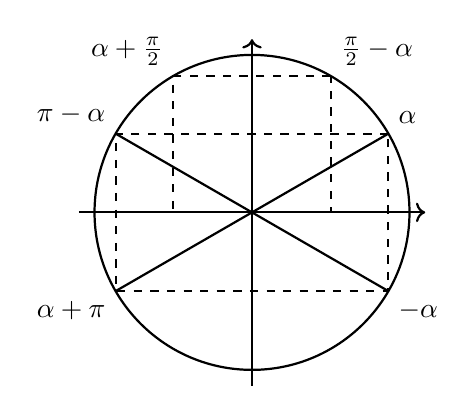
\begin{tikzpicture}[scale=2,thick]
  \draw (0,0) circle (1);
  \draw[->] (-1.1,0) -- (1.1,0);
  \draw[->] (0,-1.1) -- (0,1.1);

  \draw ({-cos(30)}, {-sin(30)}) -- ({cos(30)}, {sin(30)});
  \draw ({cos(30)}, {-sin(30)}) -- ({-cos(30)}, {sin(30)});

  \draw[dashed]
    ({cos(30)}, {sin(30)}) node[above right]{$\alpha$} --
    ({-cos(30)}, {sin(30)}) node[above left]{$\pi-\alpha$} --
    ({-cos(30)}, {-sin(30)}) node[below left]{$\alpha+\pi$} --
    ({cos(30)}, {-sin(30)}) node[below right]{$-\alpha$} --
    cycle;
  \draw[dashed]
    ({cos(60)}, {sin(60)}) node[above right]{$\frac{\pi}{2}-\alpha$} --
    ({-cos(60)}, {sin(60)}) node[above left]{$\alpha+\frac{\pi}{2}$} --
    ({-cos(60)}, {0}) --
    ({cos(60)}, {0}) --
    cycle;
\end{tikzpicture}

%--------------------------------%

%%POINTS%%%
%\tkzDrawPoint[shape=cross](A)

%%SEGMENT%%
%\tkzLabelSegment[above,below,right,left](A,B){$3~cm$}
%\tkzDrawSegments[style=dashed](A,C B,D)
%\tkzMarkSegments[mark=/](C,D)
%\tkzDrawSegment[color ={black},decorate,decoration={random steps , amplitude = 1pt}](A,B)

%%ANGLE%%
%\tkzLabelAngle[pos=0.8](B,A,C){$52^\circ$}
%\tkzMarkAngle[mark=none,size=1.1](A_2,C_2,C_3)
%\tkzMarkRightAngle(A,B,C)

%%LABELS%%
%\tkzLabelPoints(A,B)
%\tkzLabelSegment[sloped, above](I,J){$B$}
%\tkzDefCentroid(A,B,C) \tkzGetPoint{O}
%\tkzAutoLabelPoints[center=O, dist=.2](A,B,C)

%%CERCLE%%
%\draw (2,2) circle (1.5cm);

%%BOUCLE%%
%\foreach \i in {1,2,...,7}{
%    \draw (O)--(X_\i);
%}

\end{document}

%%% Local Variables:
%%% mode: LaTeX
%%% TeX-master: t
%%% End:
